% Copyright 2024 Kieran W Harvie. All rights reserved.

\topskip0pt
\vspace*{\fill}
\begin{center}
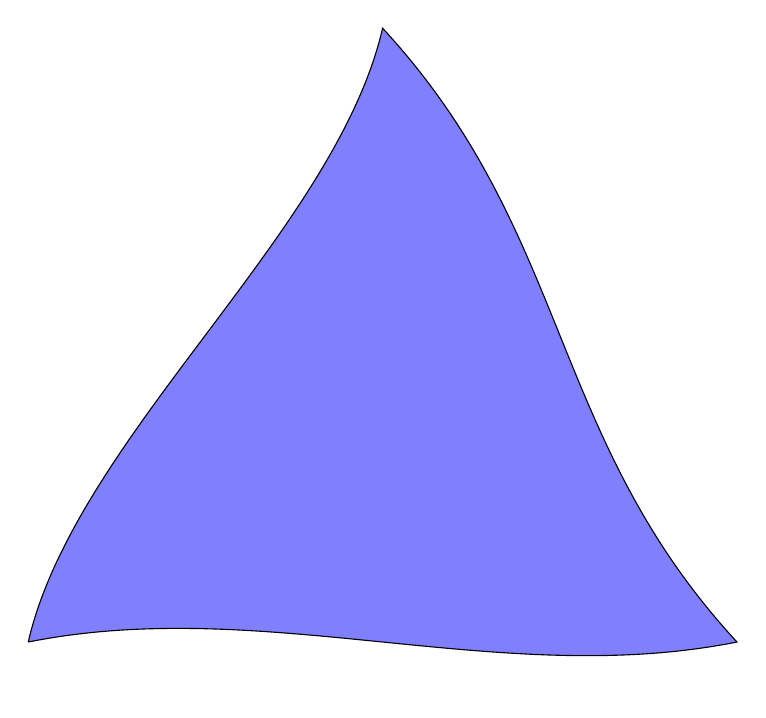
\begin{tikzpicture}[scale=1.5,every node/.style={black}]
%	\coordinate (    ) at (Y+Z*2    , Y*1.7320508075    );
	\coordinate (p300) at (0+0*2    , 0*1.7320508075    );
	\coordinate (p210) at (1+0*2-0.6, 1*1.7320508075    );
	\coordinate (p201) at (0+1*2    , 0*1.7320508075+0.4);
	\coordinate (p120) at (2+0*2+0.6, 2*1.7320508075    );
	\coordinate (p111) at (1+1*2    , 1*1.7320508075    );
	\coordinate (p102) at (0+2*2    , 0*1.7320508075-0.4);
	\coordinate (p030) at (3+0*2    , 3*1.7320508075    );
	\coordinate (p021) at (2+1*2+0.6, 2*1.7320508075    );
	\coordinate (p012) at (1+2*2-0.6, 1*1.7320508075    );
	\coordinate (p003) at (0+3*2    , 0*1.7320508075    );
	\coordinate (p300) at (0+0*2    , 0*1.7320508075    );

	\filldraw[fill=blue!50] (p300) .. controls (p210) and (p120) ..  (p030) .. controls (p021) and (p012) .. (p003) .. controls (p102) and (p201) .. (p300);
\end{tikzpicture}

An example Cubic Bézier Triangle rendered natively and easily within this very \LaTeX document.
\end{center}
\vspace*{\fill}

\newpage
